\chapter{Metodologia}
\label{cap:metodologia}

Este capítulo descreve a metodologia adotada para o desenvolvimento da aplicação. O processo será estruturado de forma a alinhar as práticas da Engenharia de Software, apresentadas na Seção~\ref{sec:engenharia_software} às particularidades do contexto do projeto. A Figura~\ref{fig:fluxo_metodologico} apresenta uma visão geral das etapas definidas.

A metodologia está organizada em seis etapas principais: (i) elicitação de requisitos por prototipação exploratória, (ii) especificação de requisitos em estrutura ágil, (iii) planejamento dos testes, (iv) modelagem do sistema, (v) desenvolvimento orientado por testes e (vi) avaliação de usabilidade.

\begin{figure}[htb]
  \caption{Fluxo metodológico do trabalho}
  \label{fig:fluxo_metodologico}
  \centering
  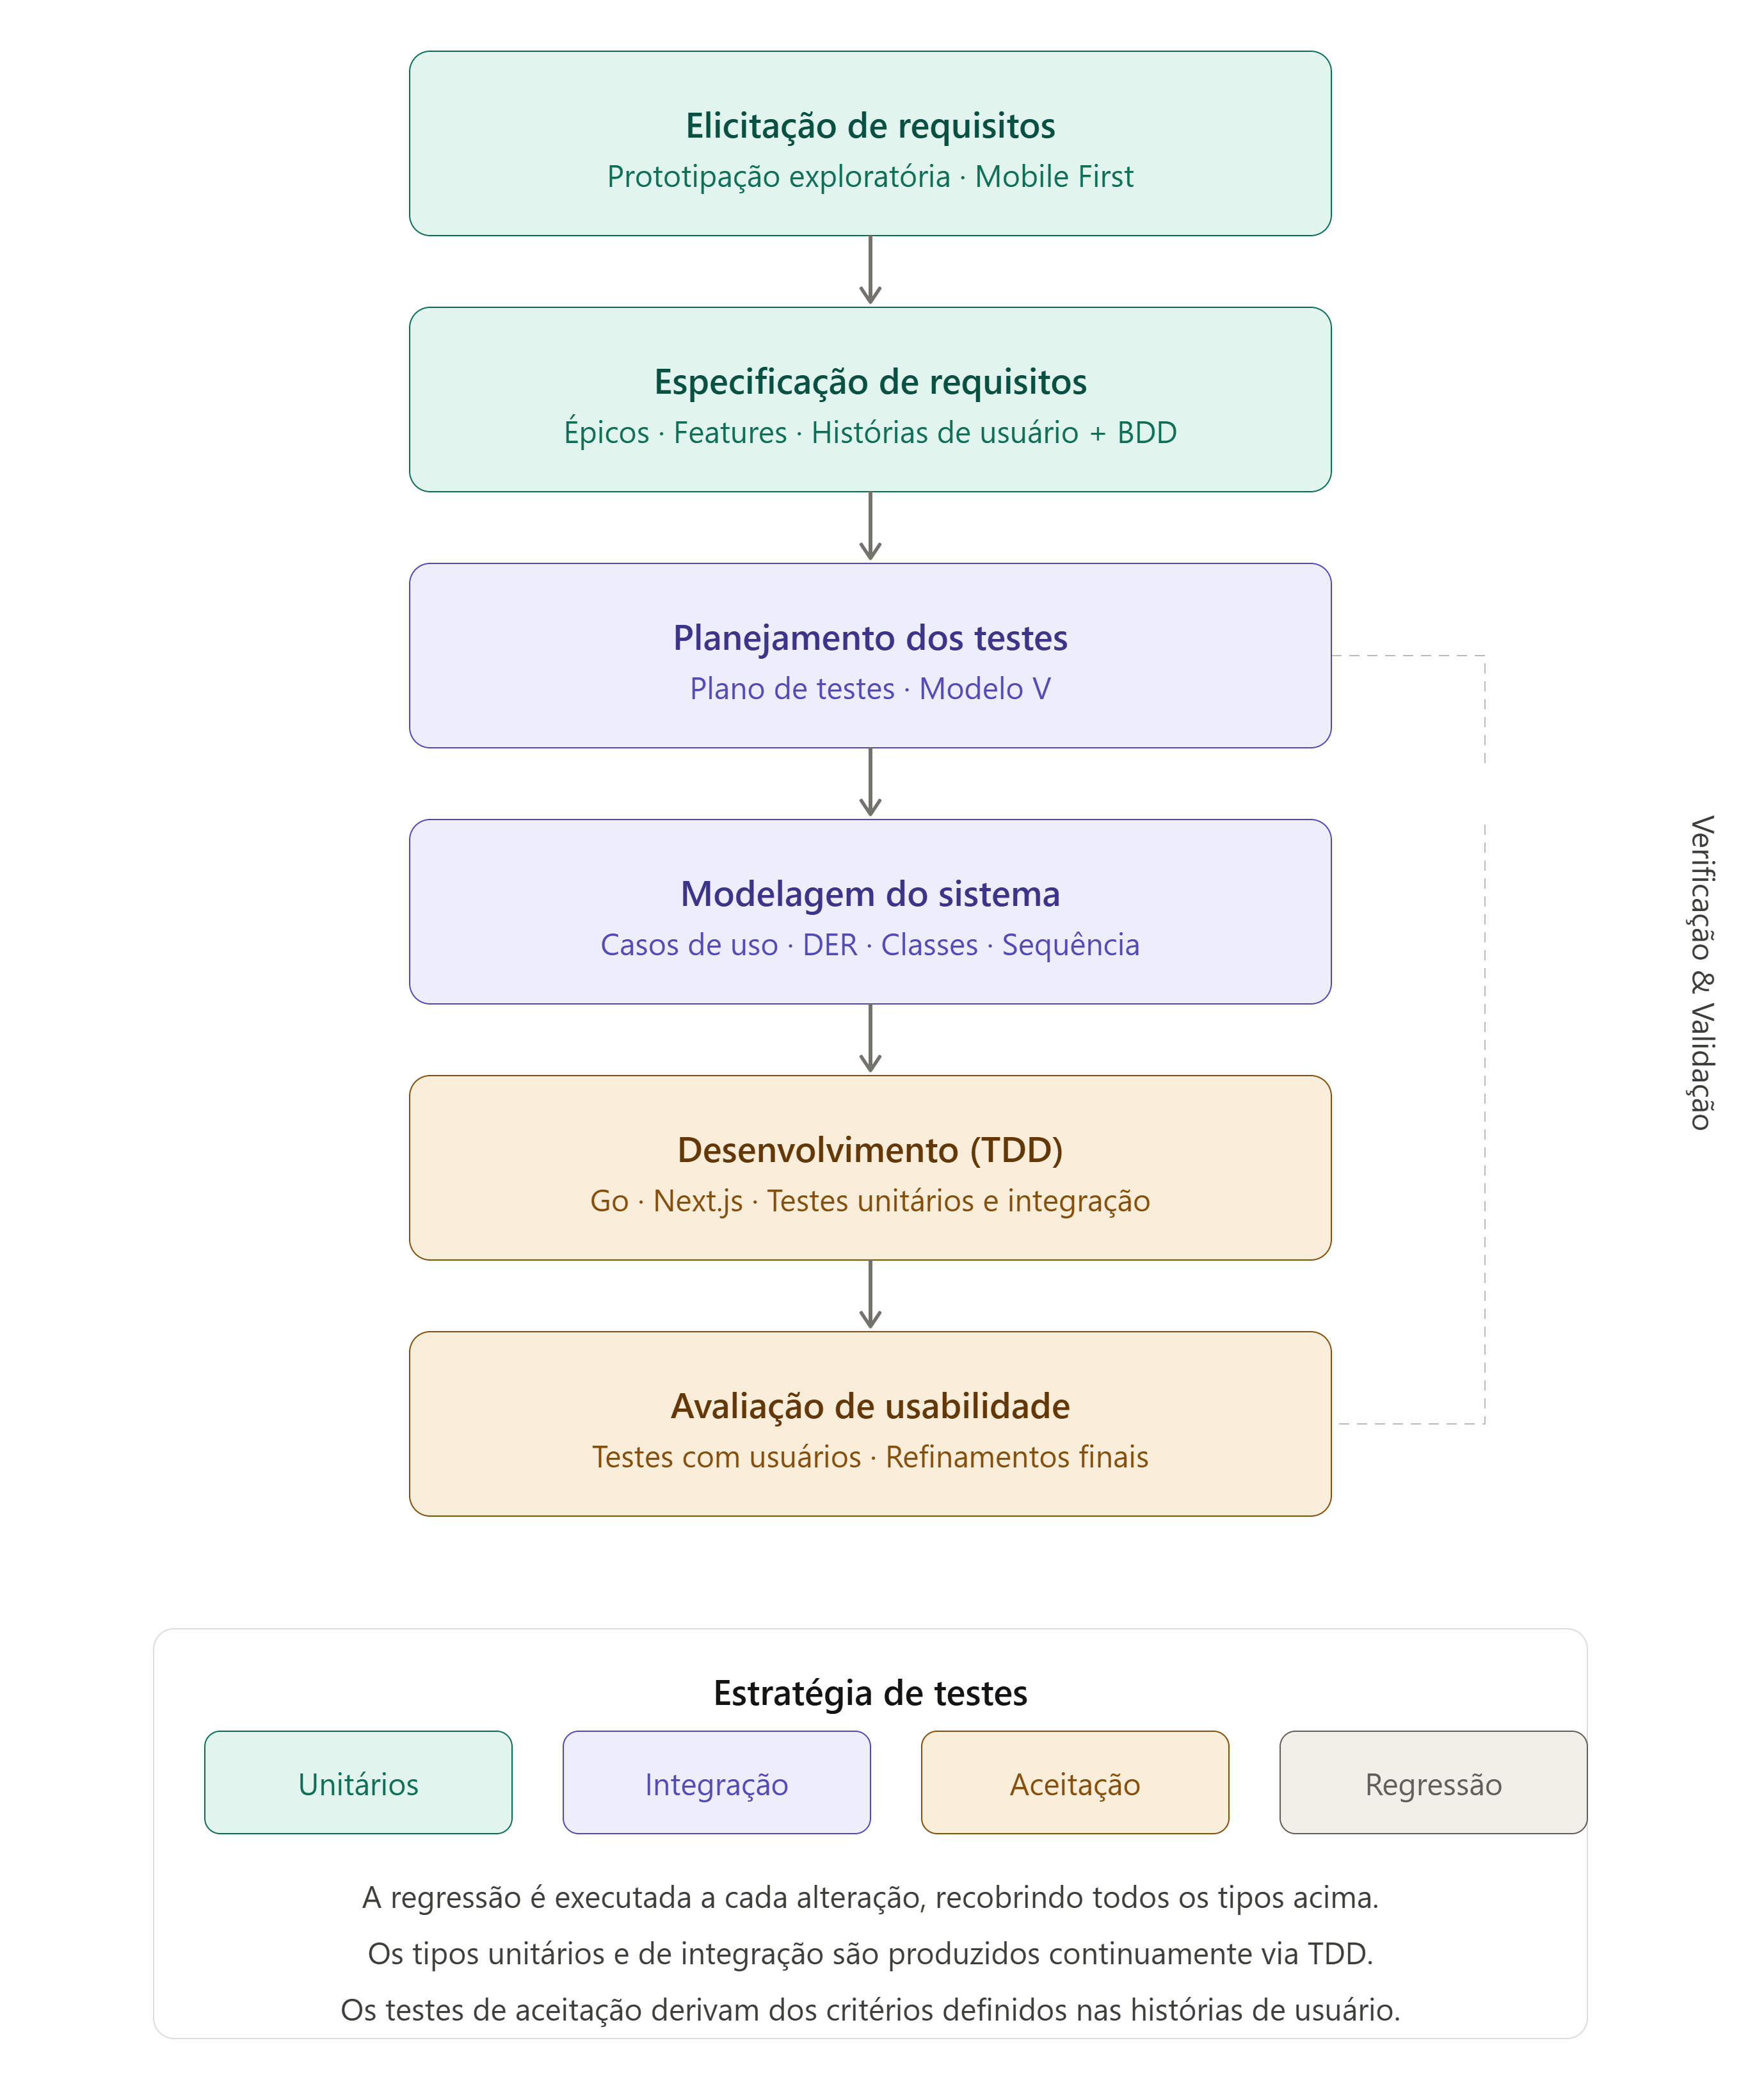
\includegraphics[width=0.8\textwidth]{figuras/fluxo_metodologico.png}

  \small Fonte: Elaborado pelo autor.
\end{figure}


\section{Elicitação de Requisitos por Prototipação Exploratória}
\label{sec:elicitacao}

A elicitação de requisitos é a etapa inicial do desenvolvimento e tem como objetivo identificar as necessidades e expectativas dos stakeholders em relação ao sistema \cite{sommerville2019}. Neste trabalho, os stakeholders envolvidos são membros da Associação de Apicultores de Poranga, caracterizados por baixa familiaridade com ferramentas digitais e por pouca experiência em processos formais de especificação de software. Esse perfil tornaria pouco eficaz a utilização de técnicas tradicionais, como entrevistas estruturadas ou formulários de levantamento de requisitos, uma vez que os usuários encontram dificuldade em expressar suas necessidades de forma abstrata, ou seja, sem uma referência visual.

Diante desse contexto, e pelas razões discutidas na Seção~\ref{sec:engenharia_software}, optou-se pela técnica de {Prototipação Exploratória} como principal estratégia de elicitação, dado que o perfil dos stakeholders deste trabalho corresponde justamente ao cenário em que essa técnica se mostra mais adequada.

Para conduzir esse processo, foram selecionados quatro stakeholders representativos. Um deles é membro com histórico de atuação em diferentes cargos da associação, possuindo uma visão abrangente dos processos internos da organização. Os demais representam um perfil para cada um dos cargos existentes, sendo eles: tesoureiro, presidente, responsável pela casa do mel e associado comum. Essa seleção intencional busca capturar tanto a perspectiva gerencial quanto a perspectiva operacional, contribuindo para uma elicitação mais completa.

Cabe destacar que, embora cada stakeholder represente um cargo distinto dentro da associação, todos eles também desempenham, em algum nível, o papel de associado comum, uma vez que utilizam as funcionalidades destinadas a esse perfil além daquelas específicas de seus respectivos cargos. Por essa razão, e por participarem ativamente da construção e da validação do protótipo ao longo de todo o processo de elicitação, espera-se que esses stakeholders apresentem, ao final dessa etapa, um nível de familiaridade com a ferramenta superior ao de um associado comum que não tenha participado do processo. Essa particularidade será retomada na Seção~\ref{sec:usabilidade}, ao tratar da avaliação de usabilidade do sistema.

O processo será conduzido em ciclos iterativos. Em cada ciclo, o protótipo será apresentado aos stakeholders selecionados, que acompanharão os fluxos de execução do protótipo por meio de explicações e perguntas constantes, de modo a estabelecer um diálogo sobre o funcionamento esperado do sistema. As observações coletadas serão analisadas e incorporadas ao protótipo na iteração seguinte. Esse processo será repetido até que os stakeholders manifestem concordância com a representação do sistema proposto, o que caracterizará a validação do protótipo como base para a especificação dos requisitos.

O protótipo será construído adotando a abordagem {Mobile First}, apresentada na Seção~\ref{sec:engenharia_software}. Essa escolha decorre da maior eficiência desse processo de design, e do fato de que apenas um dos perfis de stakeholder, o do tesoureiro, não é adequado ao uso predominante de smartphone, o que reforça a viabilidade dessa abordagem para o presente trabalho. Assim, o protótipo mobile será o instrumento utilizado durante quase todas as sessões de validação com os stakeholders. Após a aprovação final dos requisitos, será elaborado o protótipo para a versão desktop-web, utilizado como referência complementar durante a implementação.


\section{Especificação de Requisitos}

Após a conclusão das sessões de prototipação exploratória e a validação do protótipo pelos stakeholders, os requisitos do sistema serão formalizados adotando-se a hierarquia de Épicos, Features e Histórias de Usuário, e os critérios de aceitação no formato Given-When-Then, conforme apresentados na Seção~\ref{sec:engenharia_software}. Essa estrutura será adotada por facilitar a rastreabilidade entre os requisitos e os testes previstos para a etapa de desenvolvimento.

Ademais, como o stakeholder principal permanecerá disponível para consultas durante todo o projeto, a especificação será tratada como um artefato vivo, sujeito a mudanças, refinamentos e adições.


\section{Planejamento dos Testes}

Após a formalização dos requisitos, será elaborado o {Plano de Testes}, documento responsável por definir a estratégia, o escopo, os tipos de teste previstos e os critérios de qualidade adotados no projeto \cite{ieee829}. Dessa forma, o plano estabelecerá inicialmente as diretrizes gerais e os critérios de validação derivados dos requisitos, podendo ser detalhado e refinado à medida que a implementação da aplicação evoluir.

Serão adotados, neste trabalho, os quatro tipos de teste descritos na Seção~\ref{sec:vv}: unitários, de integração, de aceitação e de regressão. Os testes unitários serão produzidos de forma contínua durante o desenvolvimento, seguindo o ciclo do TDD \cite{beck2002}. Os testes de integração verificarão, em particular, a comunicação entre os \textit{handlers} da API, a camada de serviços e o banco de dados. Os testes de aceitação serão derivados diretamente dos critérios de aceitação das histórias de usuário, correspondendo à validação formal de cada funcionalidade especificada e fechando o ciclo iniciado na etapa de especificação \cite{cohn2004, north2006}. Por fim, a estratégia de regressão será especialmente relevante neste projeto, dado que novos trechos de código poderão introduzir erros capazes de afetar a confiabilidade do sistema \cite{sommerville2019}; assim, toda a suíte de testes automatizados será reexecutada sempre que uma alteração for realizada no código.

O plano de testes também registrará os critérios de cobertura adotados e as ferramentas utilizadas para execução e análise dos resultados, descritas na Seção~\ref{sec:desenvolvimento}.


\section{Modelagem do Sistema}

Com os requisitos definidos, será realizada a modelagem do sistema, conforme os princípios e a notação UML apresentados na Seção~\ref{sec:engenharia_software}. Essa etapa tem como objetivo representar a estrutura e o comportamento da aplicação antes da implementação, servindo como base para orientar o desenvolvimento e reduzir a probabilidade de decisões arquiteturais inadequadas \cite{sommerville2019}.

Neste trabalho, serão produzidos o Diagrama Entidade-Relacionamento (DER), que orientará diretamente a criação do esquema do banco de dados relacional da aplicação durante a implementação, e o Diagrama de Classes, que servirá como referência para a organização do código-fonte da API. Os Diagramas de Sequência serão elaborados seletivamente, priorizando os fluxos que envolverem múltiplos módulos da aplicação ou regras de negócio com maior risco de ambiguidade.


\section{Desenvolvimento Orientado por Testes}
\label{sec:desenvolvimento}

A implementação do sistema será conduzida seguindo a metodologia {Test-Driven Development (TDD)}, com o ciclo \textit{Red-Green-Refactor} apresentado na Seção~\ref{sec:vv} adotado como unidade básica de desenvolvimento.

A aplicação será composta por dois módulos principais: uma API REST, desenvolvida na linguagem Go, e um cliente web, desenvolvido com Next.js e TypeScript. A escolha de Go para a API justifica-se por sua tipagem estática, pela facilidade de escrita de testes unitários e de integração com a biblioteca padrão da linguagem, e pelo desempenho adequado para aplicações de gestão com múltiplos usuários concorrentes. O Next.js foi adotado para o cliente por oferecer renderização no servidor (\textit{Server-Side Rendering}), o que reduz a quantidade de processamento exigida do dispositivo do usuário ao entregar HTML pré-processado ao navegador, em vez de transferir essa responsabilidade integralmente ao cliente. Isso tornará a aplicação mais acessível em dispositivos com hardware mais limitado, como os utilizados por boa parte dos associados, alinhando-se à abordagem Mobile First adotada na etapa de prototipação. O uso de TypeScript, por sua vez, agregará tipagem estática ao desenvolvimento do cliente, contribuindo para a detecção antecipada de erros e para a manutenibilidade do código.

Os testes unitários da API serão implementados utilizando o pacote \texttt{testing} da biblioteca padrão do Go, com o auxílio de dublês de teste para isolar a camada de serviços das dependências externas. Os testes de integração serão realizados com uma instância de banco de dados de teste, verificando o comportamento completo das rotas da API desde a requisição HTTP até a persistência dos dados. Para o cliente Next.js, os testes unitários dos componentes serão implementados com as bibliotecas Jest e React Testing Library.

A suíte de testes automatizados será configurada para execução a cada alteração no código, implementando a estratégia de testes de regressão definida no plano de testes. Essa configuração garantirá que eventuais ajustes nos requisitos, decorrentes de consultas ao stakeholder durante o desenvolvimento, sejam incorporados sem comprometer as funcionalidades já validadas, além de permitir que eventuais problemas no código sejam descobertos e corrigidos rapidamente.

Os testes de aceitação serão conduzidos manualmente com base nos critérios de aceitação das histórias de usuário, verificando o comportamento do sistema integrado — API e cliente web — frente aos cenários definidos na especificação.


\section{Avaliação de Usabilidade}
\label{sec:usabilidade}

Ao término da implementação, será realizada uma avaliação de usabilidade com o objetivo de verificar se a aplicação desenvolvida atende às necessidades dos usuários de forma eficiente e satisfatória \cite{rubin2008handbook}.

Como discutido na Seção~\ref{sec:elicitacao}, os stakeholders que participaram da prototipação exploratória acompanharam de perto a evolução do sistema ao longo de todo o processo de elicitação, o que tende a torná-los usuários com maior familiaridade com a ferramenta do que um associado comum que nunca tenha tido contato com ela. Submeter a avaliação de usabilidade a esses mesmos stakeholders comprometeria a confiabilidade dos resultados, uma vez que dificuldades reais de uso poderiam não ser percebidas justamente pelo conhecimento prévio que esses participantes já possuem do sistema.

Por esse motivo, a avaliação será conduzida com associados que não participaram das sessões de prototipação, representando o perfil de usuário que terá seu primeiro contato com a ferramenta apenas após sua conclusão. Ainda que parte das funcionalidades do sistema seja destinada a cargos específicos de gestão e operação, é o uso por parte do associado comum que garante que a transparência das informações chegue de fato a todo o grupo, e não apenas àqueles que ocupam funções de liderança, sustentando assim o pilar de confiabilidade discutido anteriormente neste trabalho. Portanto, é justamente sobre esse núcleo de funcionalidades, comum a todos os associados, que a avaliação de usabilidade se concentrará.

A avaliação será conduzida por meio de Testes de Usabilidade com Usuários, conforme apresentado na Seção~\ref{sec:engenharia_software}. As tarefas serão elaboradas a partir das principais histórias de usuário relacionadas ao perfil de associado comum, cobrindo os fluxos de uso mais representativos da aplicação para esse público.

Os resultados serão analisados qualitativamente, identificando os principais pontos de dificuldade encontrados pelos usuários e as melhorias necessárias. Problemas de usabilidade identificados nessa etapa serão devidamente priorizados e, quando possível, corrigidos antes da entrega final do sistema.